\documentclass[12pt]{article}

\usepackage{sbc-template}
\usepackage{graphicx,url}
\usepackage[latin1,utf8]{inputenc}
\usepackage[brazil]{babel}
\usepackage[nonewpage]{imakeidx}
\usepackage[]{float} %Pacote que permite fazer posicionamento específico de figura com parâmetro [H]



\sloppy

\title{Modelagem de aplicativo para distribuição de informações}

\author{João Victor F. Consonni\inst{1}, Victor H. C. Leite\inst{1}, Mariana Souza\inst{1}, \\Matheus Milani\inst{1}, Artur L. Silva\inst{1}, Victor C. Denis\inst{1}, \\Bruno J. M. de Camargo\inst{1}, Danilo B. Cardoso\inst{1}, Lucas K. Kurokawa\inst{1}}

\address{Centro de Matemática, Cognição e Computação\\ Universidade Federal do ABC
  (UFABC)\\
  Av. dos Estados, 5001 - Bangú -- Santo André -- SP -- Brazil
  %\email{jconsonni, victor.costa, dantas.souza, matheus.ferreira, milani.matheus, ,artur.lazarini, v.denis , bruno.camargo, danilo.c@aluno.ufabc.edu.br}
  \email{\{jconsonni, victor.costa, milani.matheus, }
  \email{artur.lazarini, v.denis, bruno.camargo,}
  \email{danilo.c, , kenzo.kurokawa\}@aluno.ufabc.edu.br}
}
\begin{document} 

\maketitle

\begin{abstract} 
The software architecture document is essential to understand the high level structures os a software system and therefore for the decision making processes in software engineering. Here we present archtectures  based on the moldels 4+1 and C4 as part of the documentation for the system SACI - Sistema de Apoio Colaborativo de Incidentes. 
\end{abstract}

\begin{resumo} 
O documento de arquitetura de software é essencial para entender as estruturas de alto nível de um de software e, portanto, para os processos de tomada de decisão em engenharia de software. Aqui apresentamos as arquiteturas baseadas nos modelos 4 + 1 e C4 como parte da documentação do sistema SACI - Sistema de Apoio Colaborativo de Incidentes.
\end{resumo}

\section{Introdução}

A documentação de arquitetura de software traz uma abstração de altor nível do sistema a ser desenvolvido, apontando seus componentes internos e sua interação com componentes internos. Sendo assim um guia para a evolução e desenvolvimento de um sistema. Com o aumento da complexidade dos sistemas, a introdução de metologias para modelar a arquitetura desses softwares torna-se essencial para transmissão de informação para diferentes níveis de usuário destas documentações, sendo a base para tomada de decisão principalmente nas fases inciais do projeto. Para Kruchten introdução de 4 + 1, apontava que cada visão de seu modelo se adaptava à um usuário final, simplificando a visão geral do software \cite{kruchten19954+}. Já o modelo C4 de Brown, propunha uma perspectiva diferentes níveis de abstração para introdução das informações de ar quitura ao usuário \cite{C4}. Neste documento aplicamos dois modelos de arquitetura, 4 + 1 e C4, como fase do desenvolvimento do Sistema de Apoio Colaborativo de Incidentes (SACI). 




\section{Modelo 4+1}

O modelo de arquitetura 4+1 busca dividir o processo em visões concorrentes, são diferentes pontos de vista do mesmo software. A justificativa para essa abordagem é que ao fazer essa divisão a representação fica mais acessível aos stakeholders com visões que são mais de alto nível, mostrando o software de várias perspectivas que englobam visão dos usuários finais, desenvolvedores e gerentes de projeto.\cite{kruchten19954+}

Essa arquitetura apresenta 4 visões que são modeladas através de diagramas UML, sendo elas: visão lógica, visão de desenvolvimento, visão de processo e visão física. Juntas essas visões embasam a visão de cenário, que representa o +1 do modelo.

\subsection{Visão de Cenário}

A visão de cenário é composta de uma abstração que agrupa as outras 4 visões dos diagramas "4+1" e instancia os casos de uso mais genéricos, gerando de forma simplificada uma visão geral do funcionamento dos requisitos mais importantes do sistema. A visão de cenário também tem o intuito de  auxiliar as fases de teste, durante e depois da implementação do sistema.

O diagrama a seguir representa um compilado dos casos de uso apresentados no documento de diagramas da entrega 2.

\begin{figure}[!h]
    \center{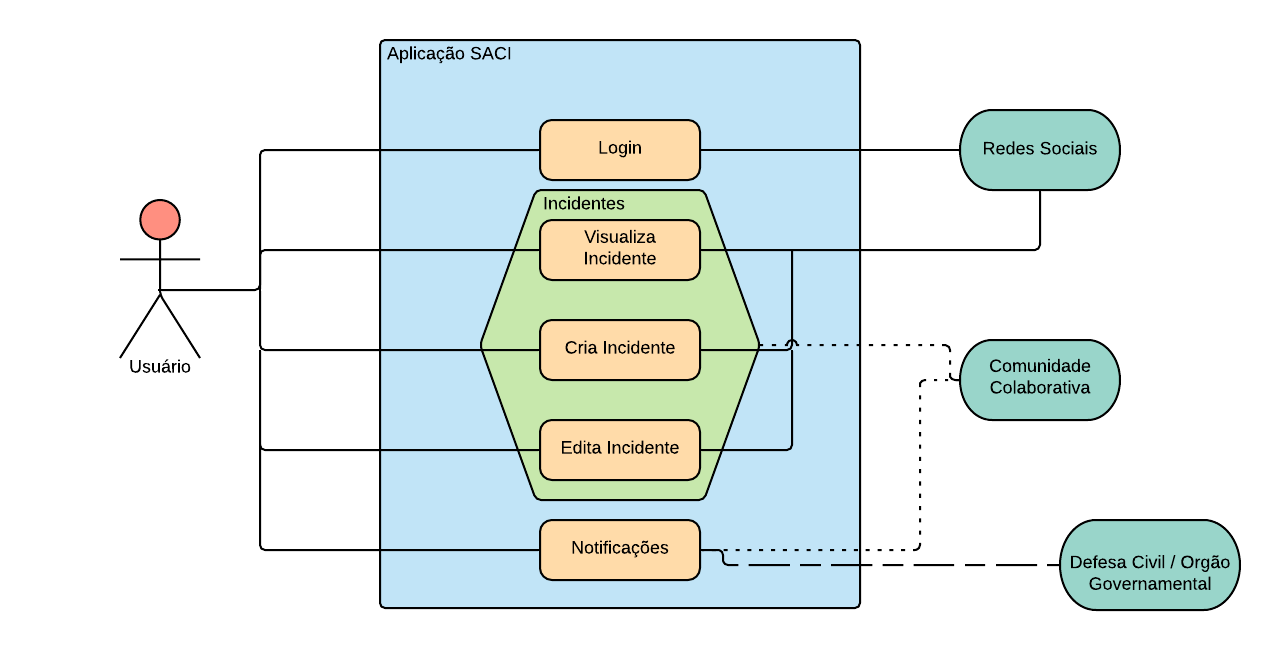
\includegraphics[width=\textwidth]
    {imagens/"ArcModel4+1"/CasodeusoSaci.png}}
    \caption{\label{fig:casoUso} Modelo de Arquitetura 4+1 - Diagrama de Caso de uso - Visão de Cenário}
\end{figure}

\vfill% para consertar pagebreak
\pagebreak%Quebra de página para consertar imagens

\subsection{Visão Física}

A visão física consiste em aplicar os requisitos não funcionais do sistema, ligando o hardware com o software a ser implementado. Este mapeamento entretanto serve para nortear o desenvolvimento do software, tendo em si um pequeno impacto no código a ser implementado.


\begin{figure}[!h]
    \center{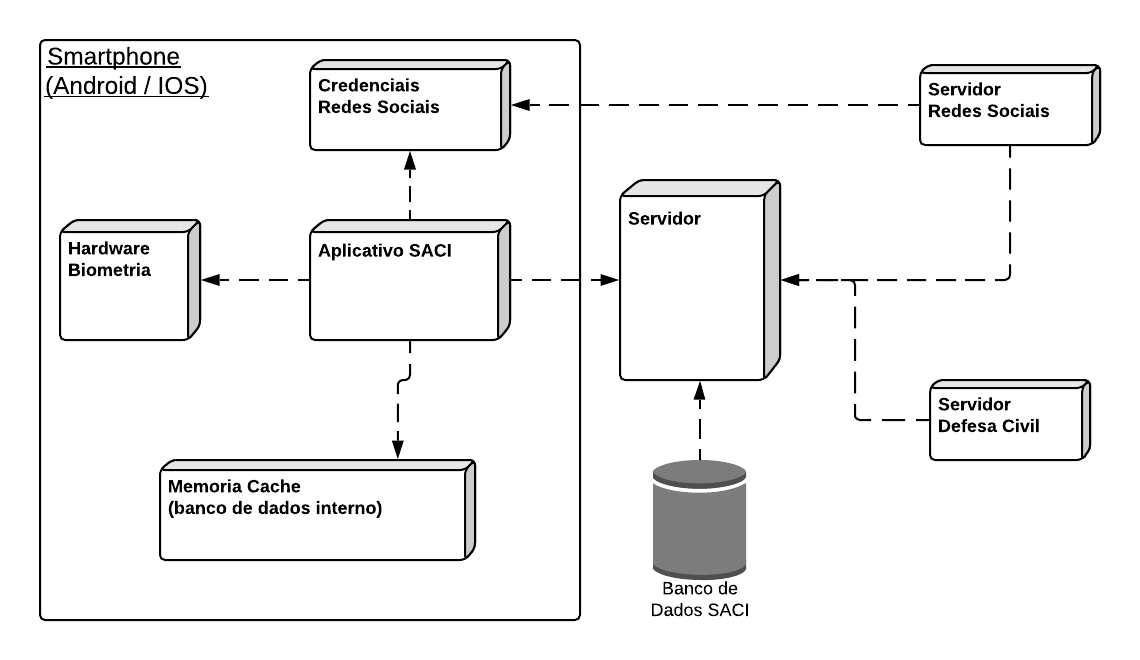
\includegraphics[width=\textwidth]
    {imagens/"ArcModel4+1"/VisaoFisica.png}}
    \caption{\label{fig:visaoFisica} Modelo de Arquitetura 4+1 - Diagrama de Hardware - Visão Física}
\end{figure}

\vfill%vfill para consertar pagebreak
\pagebreak%Quebra de página para consertar imagens

\subsection{Visão de Processo}

A visão de processo busca descrever como ocorrem as atividades da aplicação, descrevendo qual a ordem dos processos e como ocorre a comunicação entre eles através da estrutura de elementos de execução. Ela facilita o entendimento de como a informação é tratada dentro da aplicação representando os principais componentes e suas interações.
Para modelar essa visão foi utilizado o diagrama de atividades a seguir, o diagrama mostra o fluxo principal de atividade da aplicação (porém não todo o fluxo). O diagrama contempla os requisitos a seguir: RC02, RC03, RC04, RC05, RC06, RC07, RC09, RC20, TI01, TP01, TP02, TP09, TP11 e VI01.

\begin{figure}[!h]
    \center{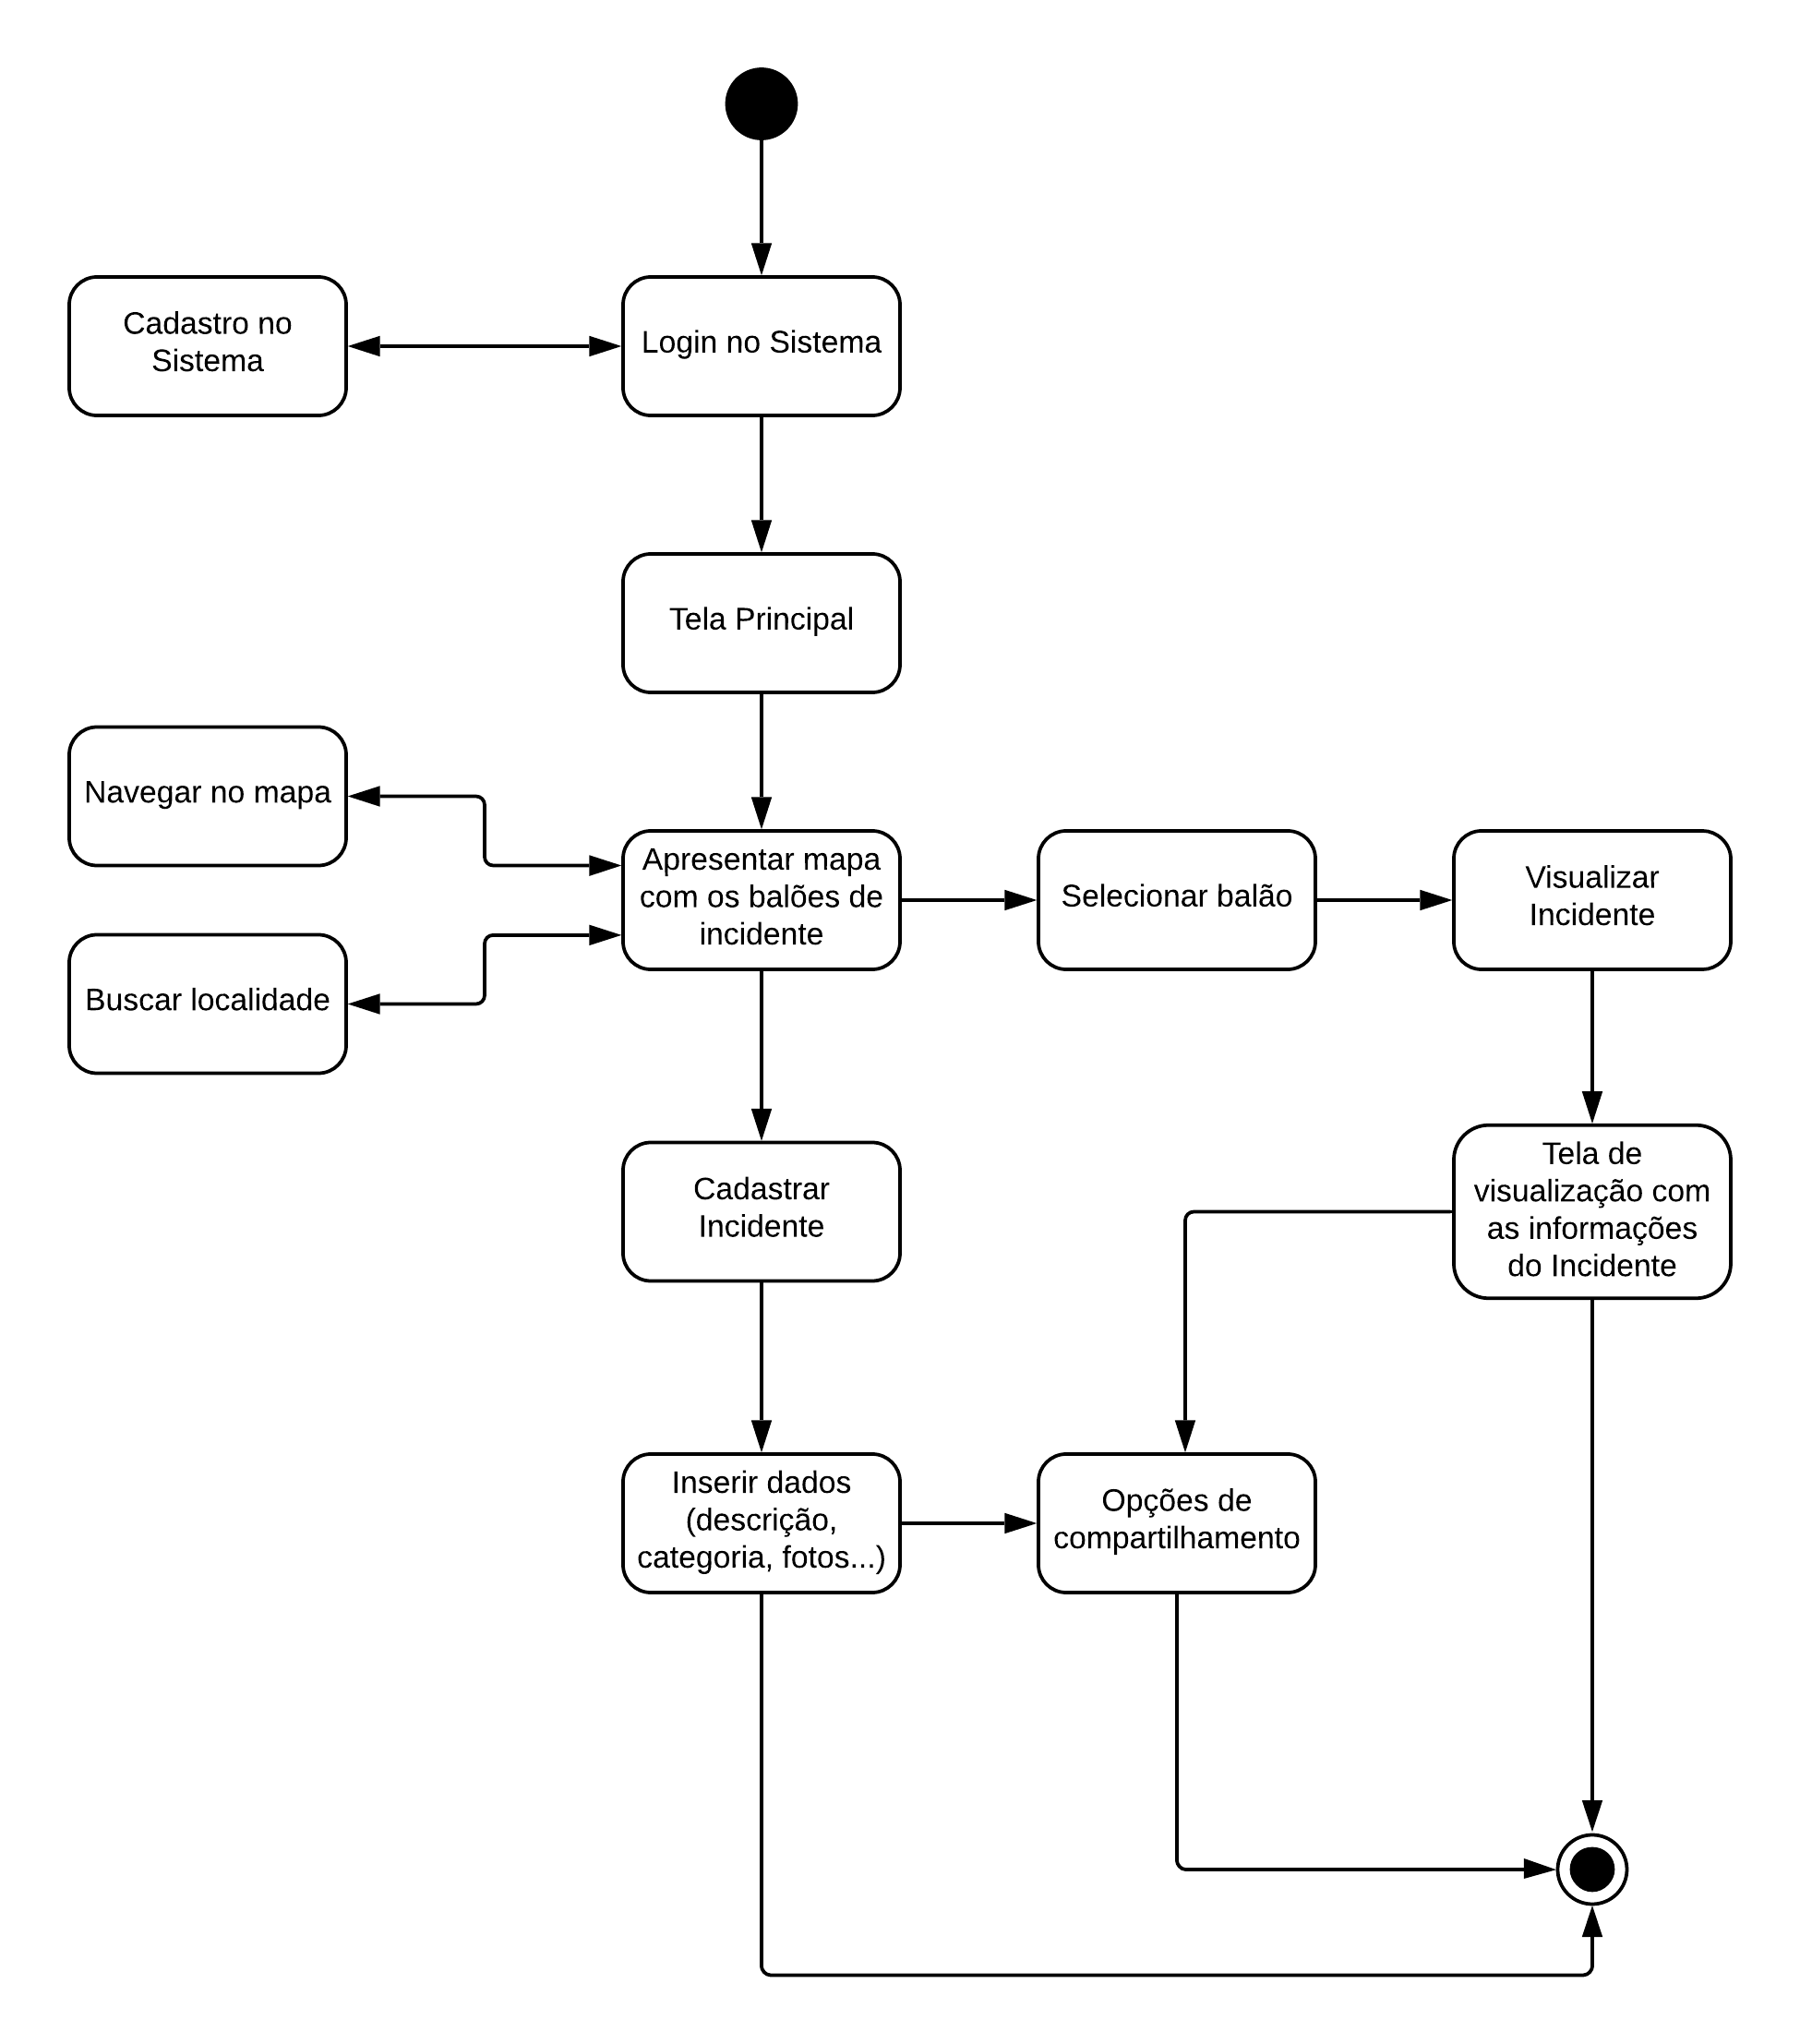
\includegraphics[width=\textwidth]
    {imagens/"ArcModel4+1"/processView.png}}
    \caption{\label{fig:processView} Modelo de Arquitetura 4+1 - Diagrama de Atividade - Visão de Processo}
\end{figure}

\vfill%vfill para consertar pagebreak
\pagebreak%Quebra de página para consertar imagens

\subsection{Visão de Desenvolvimento}

O diagrama a seguir demonstra como os componentes do sistema SACI se relacionam, pois esta visão ajuda as pessoas a entenderem como funciona a estrutura e as interdependências dos sistemas englobados.

  \begin{figure}[!htb]
    \center{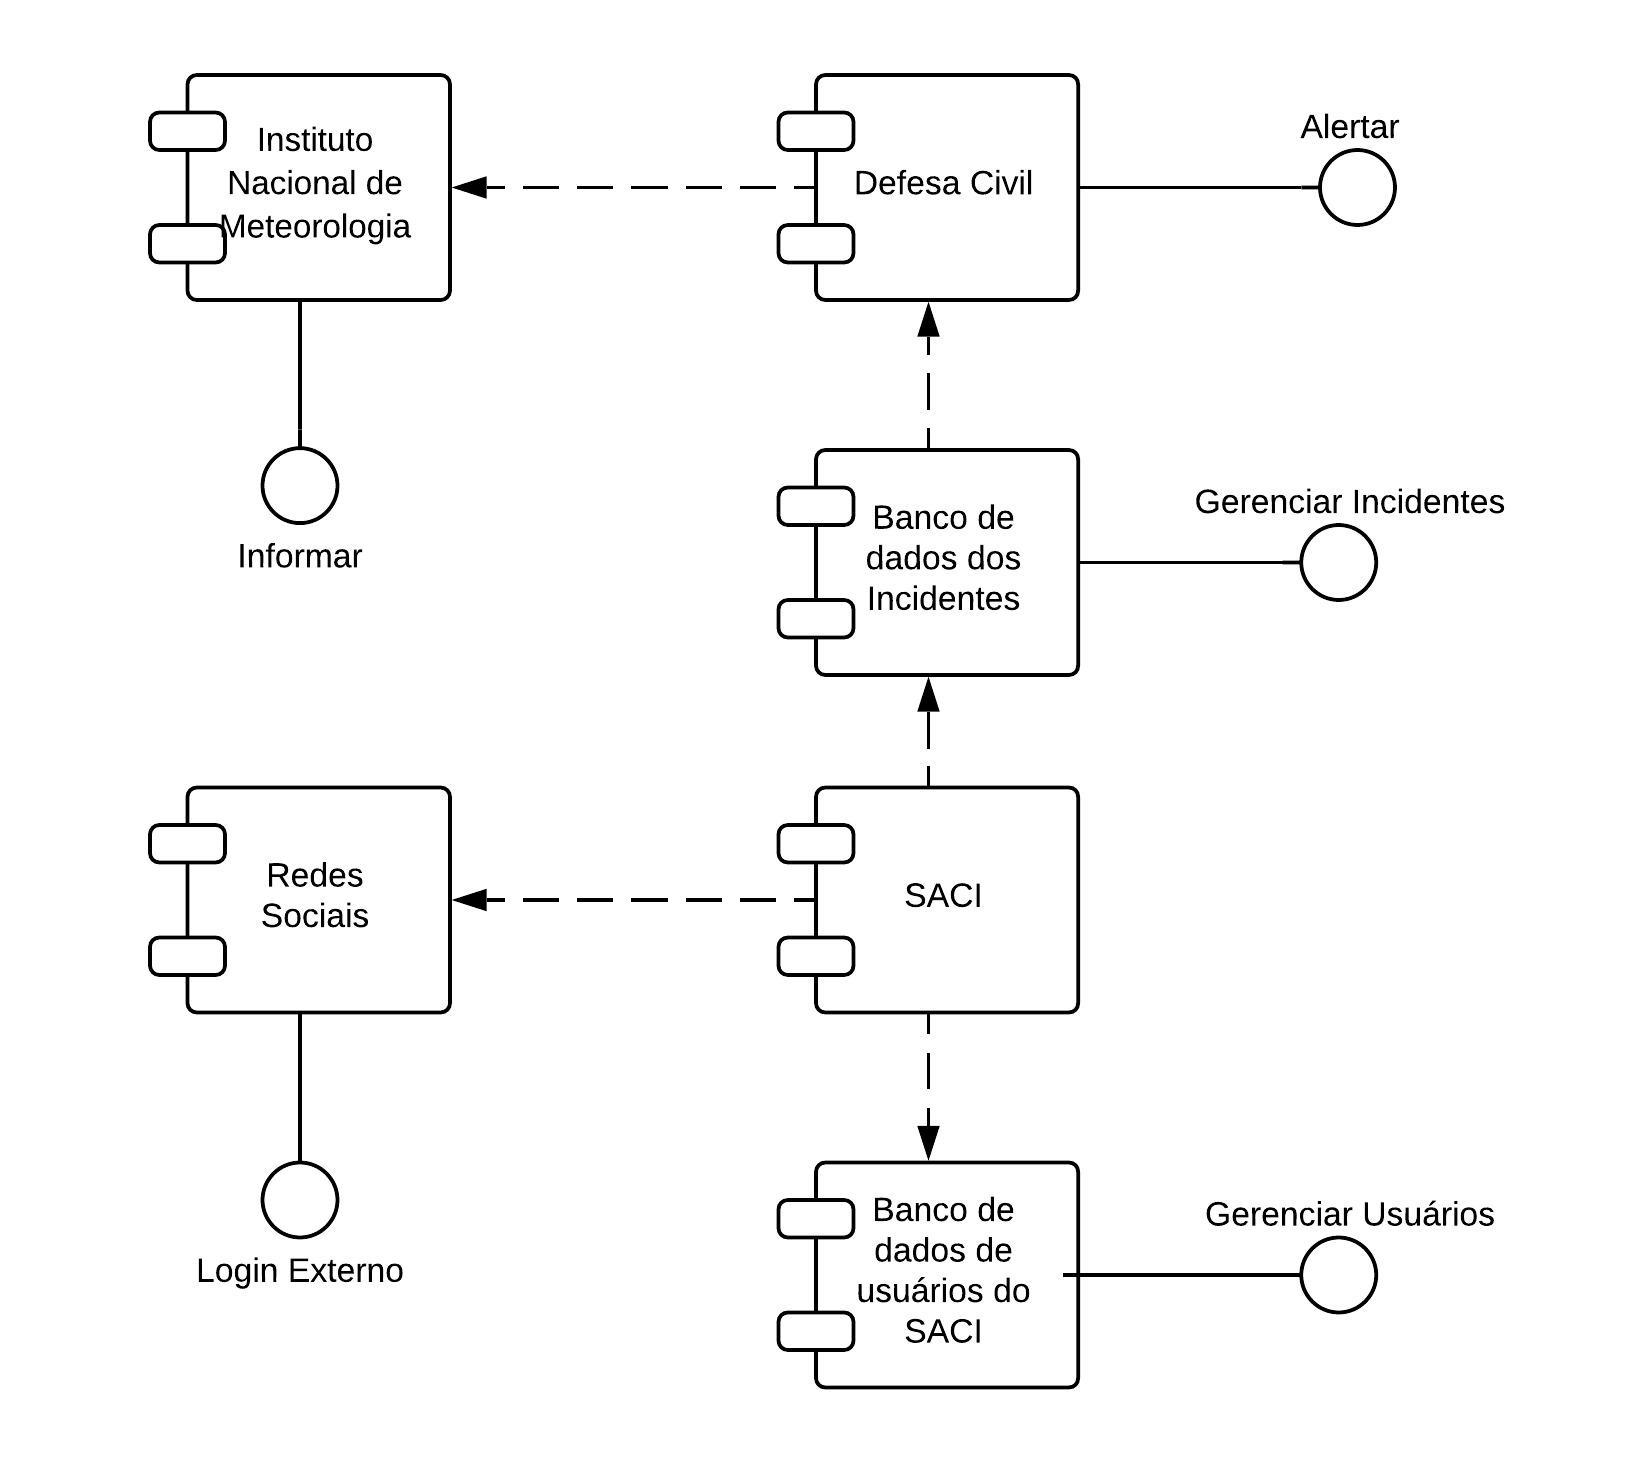
\includegraphics[width=\textwidth]
    {imagens/DiagramaComponentes/diagramaComponente.png}}
    \caption{\label{fig:diagComponentes} Diagrama de Componentes}
  \end{figure}

\vfill%vfill para consertar pagebreak
\pagebreak%Quebra de página para consertar imagens

\subsection{Visão Lógica}

A visão lógica representa as entidades do sistema, mostrando as classes e o modelo de banco de dados. Também pode exibir funcionalidades que o sistema disponibilizara para o usuário final. Os diagramas UML usados para representar a visão lógica incluem: Diagrama de classes, Diagrama de comunicação e Diagrama de sequencia.
Nós modelamos a visão através do diagrama de classe a a seguir. O diagrama de classe aborda todos os requisitos que estão relacionados com os dados que a aplicação processa ou armazena.

\begin{figure}[!h]
    \center{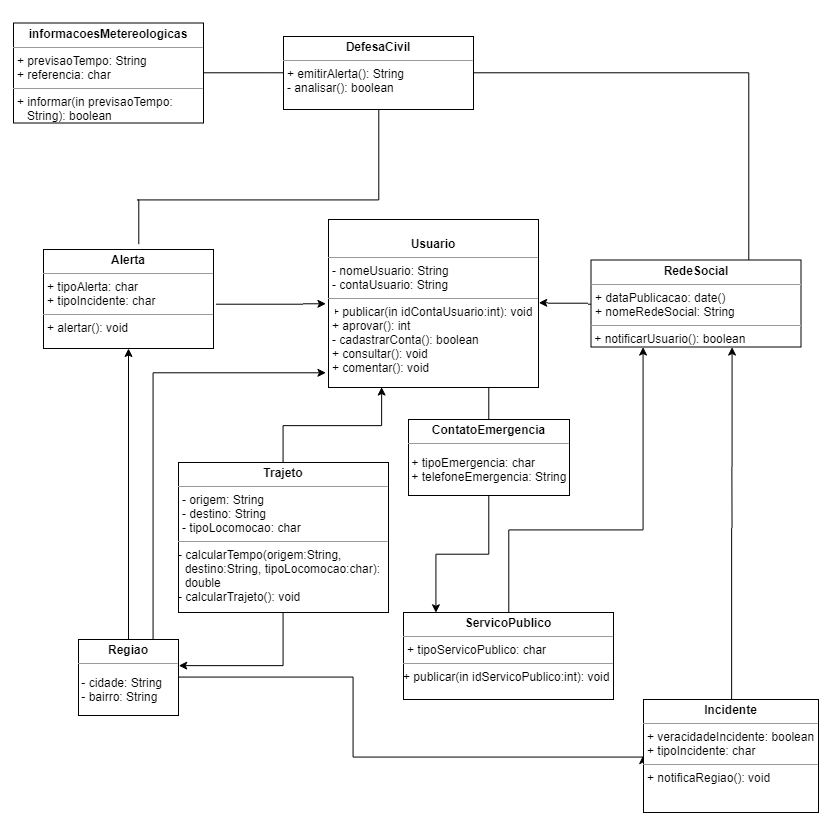
\includegraphics[width=\textwidth]
    {imagens/diagClasses.png}}
    \caption{\label{fig:DiagClasse} Modelo de Arquitetura 4+1 - Diagrama de Classe - Visão Lógica}
\end{figure}

\vfill%vfill para consertar pagebreak
\pagebreak%Quebra de página para consertar imagens

\section{Modelo C4}
O modelo de representação de arquitetura de software C4, sigla para "\textit{Context, Container, Component, Code"}, visa otimizar um dos \textit{side-effects} negativos advindos das metodologias ágeis de processos de desenvolvimento, a representação da arquitetura do software. 

De forma simplificada, o modelo tenta mergulhar em diferentes níveis de abstração em cada um dos "C", que resultam em diagramas que documentam desde como a aplicação é inserida no contexto dos seus usuários e seu ecossistema, até níveis mais baixos, demonstrando relacionamentos entre componentes internos do software e, possivelmente, até chegar a nível de código de implementação.

O grupo idealizou o sistema na tentativa de seguir a estrutura de código pregada pelo padrão MVC, portanto, visualizou-se a separação de seções do código em categorias como Models, Controllers e Views.
A partir desta discussão, definiu-se de maneira superficial, o conteúdo de cada diagrama.

Em um primeiro momento o grupo enfrentou algumas dificuldades em interpretar os conceitos de contexto, contêiner e componente utilizados pelo modelo C4 e como ficaria a de fato a representação final, o que gerou mais discussão, por exemplo, como ficariam distribuídos os componentes e o que faria mais sentido sem exibido em qual diagrama. Adicionalmente, para o grupo, ficou um pouco abstrato demais tratar a estrutura de código como MVC para uma aplicação móvel sem ter muita experiencia prática de fato com o conceito.

Em contra partida, escolheu-se o MVC como ponto de partida pois conceitualmente é de fácil visualização e define boas convenções a serem seguidas quanto ao isolamento de responsabilidades das diferentes frações de uma aplicação, tornando o código mais modularizado e de fácil manutenibilidade.

% =====================================================

% \textbf{To-Do}
% \begin{enumerate}
%     \item Requisitos contemplados e não contemplados? Faz sentido???
% \end{enumerate}

% =====================================================

\subsection{Contexto}
O Diagrama de Contexto mostra de maneira geral o sistema, sem aprofundar em detalhes técnicos. Este tipo de diagrama é utilizado para mostrar a arquitetura do sistema com foco em representar as interações com seus usuários sendo assim uma visão de alto nível da arquitetura.

\begin{figure}[!h]
    \center{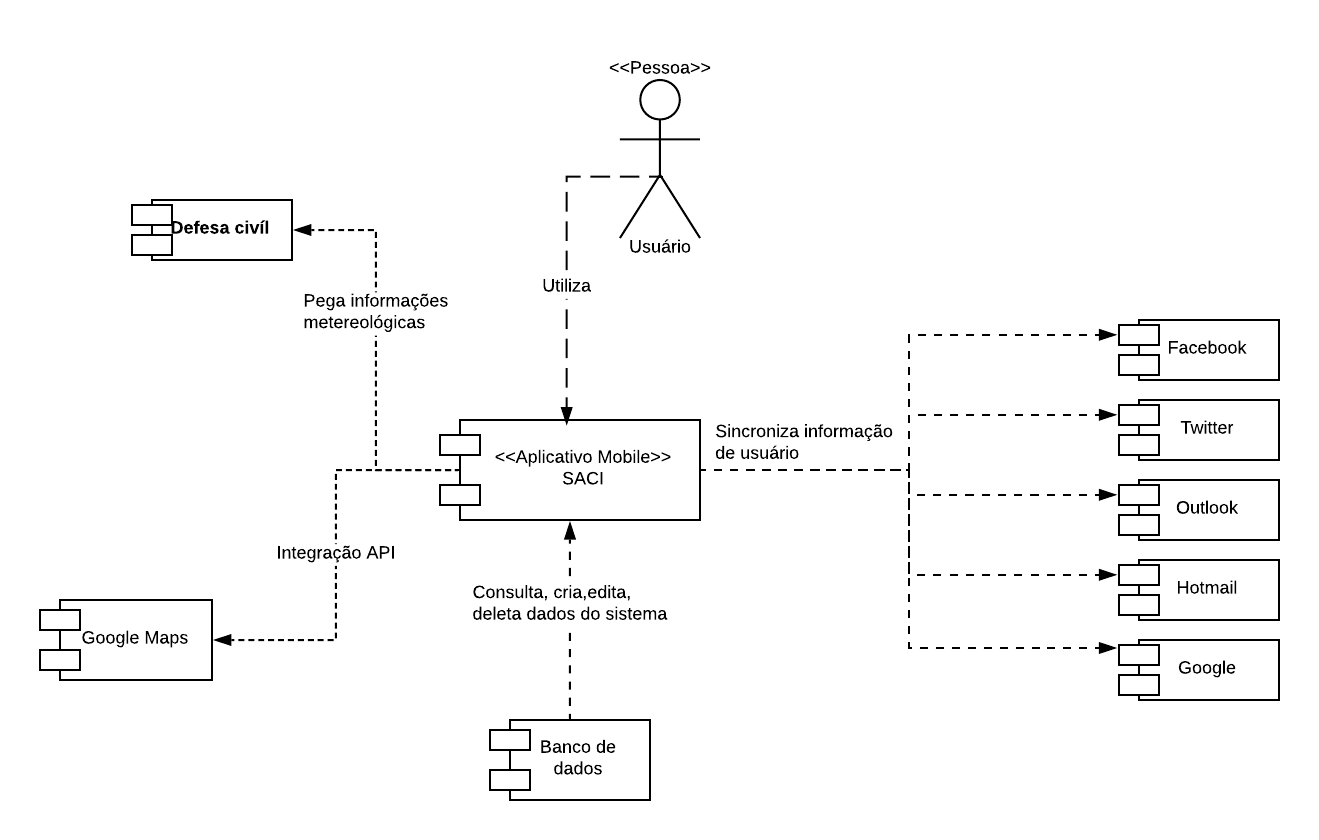
\includegraphics[width=\textwidth]
    {imagens/"c4 diagrams"/Context.png}}
    \caption{\label{fig:diagContexto} Diagrama de Contexto}
\end{figure}
\vfill%vfill para consertar pagebreak


\pagebreak%Quebra de página para consertar imagens


\subsection{Containers}
O Diagrama de Contêineres descreve um nível menos abstrato que o de contexto. Ele é utilizado por desenvolvedores do software e times de suporte levando uma visão de alto nível do software. Ele demonstra como o software se comporta e com quais sistemas ele se conecta além dos sistemas do próprio software.

\begin{figure}[!h]
    \center{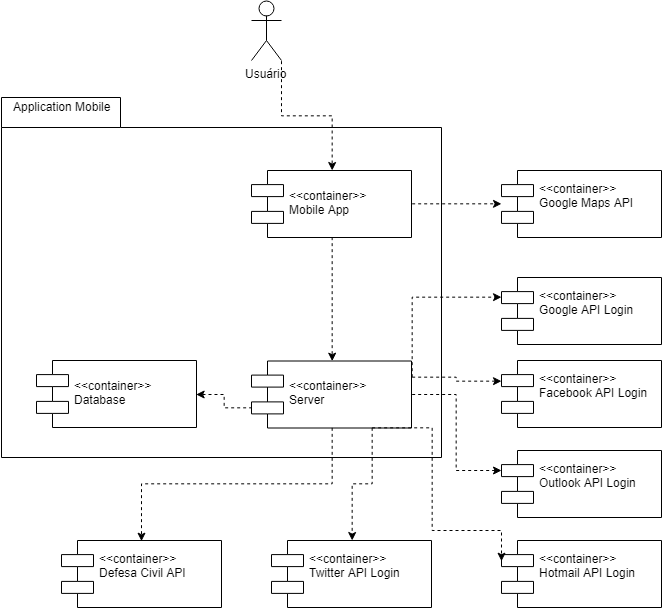
\includegraphics[width=\textwidth]
    {imagens/"c4 diagrams"/Server_Container.png}}
    \caption{\label{fig:diagContainer} Diagrama de Containers}
\end{figure}
\vfill%vfill para consertar pagebreak


\pagebreak%Quebra de página para consertar imagens


\subsection{Componentes}
O diagrama de componentes aprofunda em mais um nível de abstração, adentrando o escopo interno dos contêineres. Desta forma é possível representar como aquele contêiner é constituído, quais componentes estão inclusos em seu escopo e como é a a interação entre estes componentes. Pode-se especificar em mais detalhes as tecnologias utilizadas e uma visão geral de implementação.

Neste diagrama vemos a como a aplicação seria estruturada em um nível um pouco mais baixo. Neste contexto, conseguimos ver as estruturas idealizadas da arquitetura MVC. Temos um conjunto de modelos (Models), que são responsáveis por orquestrarem a interface aplicação/banco de dados. São representações das entidades do contexto da aplicação, sendo que cada instancia desses modelos representam uma linha da respectiva tabela no banco de dados e cada atributo corresponde à uma coluna da mesma tabela.

Relacionados a estes modelos temos os controladores (Controllers). Serão estas classes que encapsularão grande parte da logica da aplicação. Baseando-se na interação do usuário com a interface do aplicativo, os Controllers decidem o que deve ser feito com os dados recebidos, podendo desde invocar os Models para ler/escrever dados armazenados, até  efetuarem alguma lógica interna que represente uma feature/regra de negócio da aplicação. Quando uma resposta desse processamento é obtida, os Controller se encarregam de invocarem a interface correta (Views) para que o ciclo de interação com usuário continue.

Desta forma, visualizamos a aplicação com uma seção responsável pelo fluxo de cadastro e acesso à aplicação pelos usuários (LoginController, SessionController, UserModel), outra para os fluxos relacionados ao gerenciamento e compartilhamento de incidentes (IncidentController, IncidentModel e Views correspondentes) e por fim uma seção ressonável pelo gerenciamento de alertas baseados nas informação coletadas, tanto internamente, quanto externamente através da comunicação com centrais de medições e com bases da Defesa Civil.


\begin{figure}[!h]
    \center{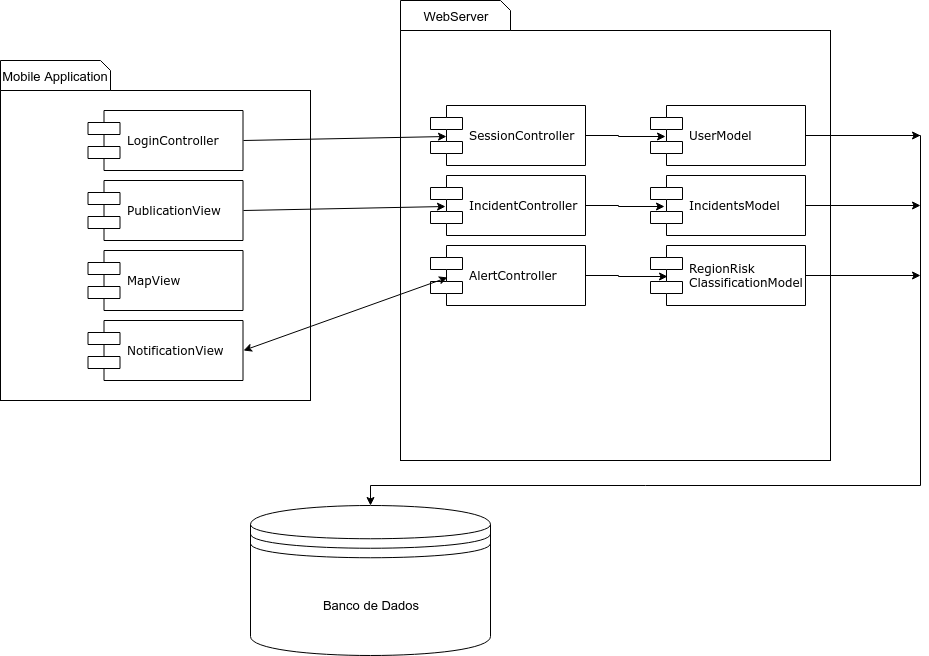
\includegraphics[width=\textwidth]
    {imagens/"c4 diagrams"/Components.png}}
    \caption{\label{fig:diagC4Components} Diagrama de componentes}
\end{figure}
\vfill%vfill para consertar pagebreak

\pagebreak%Quebra de página para consertar imagens

\section{Discussão}
Nasta etapa do projeto, foi desenvolvida a arquitetura de software com base em dois modelos arquiteturais: 4+1 e C4. Ambos utilizaram como referência os diagramas construídos na etapa anterior, assim como o documento de requisitos.

Durante este processo ficou evidente a interrelação entre cada um dos documentos desenvolvidos até então, assim como a importância da criação destes artefatos como forma de centralizar e elucidar todas as informações necessárias ao desenvolvimento do software, permitindo, assim, maior coerência das funcionalidades e organização do produto. Além disso, a elaboração destes documento consiste uma etapa importante para garantir a difusão do conhecimento dentor da equipe, assim como concordância das suas características.

Para as próximas fases de projeto, este documento, assim como os documentos anteriores, terão o importante papel de facilitar a comunicação tanto entre os membros da equipe, quanto com o cliente.

\section{Conclusão}
O processo de elaboração da arquitetura do software, baseada em modelos bem consolidados e concisos, foi bastante enriquecedora para a percepção de quão complexo é o processo de desenvolvimento de um software. Um produto aparentemente simples, como o que estamos desenvolvendo, já requer um volume bastante grande especificações, de forma a tornar possível a sua implementação planejada, reduzindo o risco do projeto e eventuais custos com retrabalho.

Para garantir a qualidade do software e a satisfação do cliente, o processo de documentação e modelagem agrega um valor difícil de ser mensurado, mas ainda assim evidente, principalmente para aqueles envolvidos no processo de criação em si. Documentos como este ajudam a definir o produto. Quando há clareza quanto ao “o quê” deve ser desenvolvido, o processo se torna mais fluido e menos desgastante. Desta forma, o conjunto dos documentos produzidos até então constituem uma base sólida para a criação do nosso produto.

\section{Como o processo de Scrum foi seguido pela equipe}
Por tratar-se de um fluxo incremental e iterativo, o processo SCRUM é ideal para a elaboração de documentos que devem, justamente, definir do que se trata o produto. No início, as funcionalidades, do produto ainda estão em um estado abstrato e as ideias a respeito do que o produto faz, e o que não faz, estão, de certa forma, difusas. A cada sprint, o produto ganha mais forma, ficando mais claro na mente da equipe.

O Trello mostrou-se uma ferramenta fundamental para a divisão de tarefas, assim como para a centralização dos artefatos produzidos e rastreamento do andamento de atividades. Nessa sprint, em específico, o Whatsapp teve um papel excencial na comunicação. Diferente do que foi feito nas sprints anteriores, em que cada membro tinha tarefas que eram, em certo grau, independentes, nesta sprint os modelos arquiteturais foram divididos em duas equipes. Os membros de cada equipe tiveram que trabalhar em conjunto para produzir cada modelo, o que exigiu sincronismo e comunicação frequente. 

Além disso, os novos membros se adaptaram bem à equipe e contribuíram bastante com o produto. A troca dos integrantes que assumiram os papeis de Scrum Master e Project Owner teve pouco impacto na produtividade da equipe em si, não a afetando perceptivelmente, o que pode ser considerado positivo, pois a produtividade da equipe, que já era muito boa, foi mantida, mesmo com o abalo da mudança na equipe.

O Scrum já está se tornando mais fácil de ser implementado, uma vez que os mebros estão cada vez mais familiares a ele. As reuniões de retrospectiva e review tem ajudado a revisar nossos métodos e a superar nossas dificuldades, como o inicial desconhecimento das ferramentas (Trello, Overleaf, etc.) por parte de alguns membros. A planning foi fundamental para estruturar as tarefas e dividi-la na equipe. 


\bibliographystyle{sbc}
\bibliography{main}

\end{document}